%------------------------------------------------------------------------------------
%	CHAPTER 1
%------------------------------------------------------------------------------------
\chapterimage{headerCap.png}
\chapter{Conceitos Introdutórios}

\begin{remark}
A filosofia do Linux é ``Ria na face do perigo''. Opa. Errado. ``Faça você mesmo''. É, é essa. (Linus Torvalds) 
\end{remark}

\section{Do que trata esse livro?}\index{Conceitos Introdutórios}

Assim como eu, resolveu mudar para o Linux e se encontra um tanto perdido, ou está aborrecido com seu sistema operacional e deseja usar o Linux mas tem medo de migrar por causa dos seus aplicativos, ou já usa o Linux mas ainda está perdido? Não se preocupe isso acontece com todos desde o mais leigo até o mais experiente.

Era um usuário do Windows e principalmente do MS-Office, sabia usar o Excel na perfeição, craque no Word e melhor ainda o PowerPoint, e isso inclui três coisas que muito poucas pessoas fazem: \vspace{-1em}
\begin{itemize}[noitemsep]
 \item Uso de Macros;
 \item Composição da Mala Direta; e 
 \item Integração OLE dos aplicativos.
\end{itemize}

Por causa do trabalho, tive que mudar para o \textbf{OpenOffice}\footnote{No Brasil teve que se chamar BR Office devido a direitos legais} foi nessa hora que pensei ``meu mundo caiu''. Tinha duas escolhas, a primeira era pedir demissão e a segunda aprender esse novo ambiente. Como toda pessoa inteligente que encara os problemas como desafios e oportunidades agarrei o momento para começar minha mudança para o \textbf{Software Livre} - que na época achava que era apenas grátis.

Existem grandes diferenças entre Software Livre e Software Grátis (ou \textit{Freeware}). Grátis significa que se pode copiar e usar um determinado software sem ter que pagar um centavo para ninguém, porém sem a disponibilização de seu código-fonte nem o poder de modificá-lo. Já o Software Livre está associado a quatro liberdades básicas.

Tudo começou porque um programador chamado \textbf{Richard Matthew Stallman} teve um problema com o software em sua impressora. Ele mesmo poderia consertar mas não estava autorizado a modificar ou mesmo olhar o código-fonte do fornecedor.

Stallman então criou as regras para o chamado Software Livre, foi o fundador do movimento Software Livre, do projeto GNU\footnote{Um sistema operacional tipo Unix cujo objetivo é oferecer um sistema totalmente composto por software livre}, e da FSF\footnote{Free Software Foundation é uma organização sem fins lucrativos} dedicada ao desenvolvimento colaborativo e a divulgação do Software Livre. Também é o autor da GPL\footnote{General Public License}, a licença livre mais utilizada no mundo, que garante a total distribuição do código-fonte e impede que o mesmo se torne parte de um Software Proprietário.

Ao se utilizar de qualquer Software Livre o usuário, segundo Stallman, tem direito a quatro liberdades básicas: \vspace{-1em}
\begin{itemize}[noitemsep]
 \item A liberdade de executar o programa, para qualquer propósito (liberdade nº 0)
 \item A liberdade de estudar como o programa funciona, e adaptá-lo para as suas necessidades (liberdade nº 1). Acesso ao código-fonte é um pré-requisito para esta liberdade.
 \item A liberdade de redistribuir cópias de modo que você possa ajudar ao seu próximo (liberdade nº 2).
 \item A liberdade de aperfeiçoar o programa, e liberar os seus aperfeiçoamentos, de modo que toda a comunidade se beneficie (liberdade nº 3). Acesso ao código-fonte é um pré-requisito para esta liberdade.
\end{itemize}

Ou seja, um Software Grátis não é necessariamente livre, mas um Software Livre é sempre Grátis. E principalmente teria os fontes na minha mão para estudar, foi essa ideia que me atraiu, não tive dúvidas e cai de cabeça nesse novo mundo. Não foi fácil me readaptar (como nunca é), mas tive grandes vantagens nesse processo.

Escrevi esse livro como um modo de ajudar a qualquer um que esteja no mundo Linux, usa a distribuição Ubuntu\footnote{Acredito que muitos detalhes neste livro pode ser aproveitado para diversas outras distribuições, principalmente nos filhos do Ubuntu} e deseja se adaptar da melhor forma. Use-o para instalar e montar um ambiente tranquilo para usar seu computador como melhor lhe agrada. Resumidamente, usar o Linux e descobrir que o pinguim está mais do que domesticado e pode ser usado sem problemas seja em casa ou no trabalho.

\section{Por que o símbolo do Linux é um Pinguim?}\index{Conceitos Introdutórios}
Acredito que todo livro que fala a respeito do Linux conta da sua mascote o pinguim com o nome de \textbf{Tux}, ou seja, essa história já foi contada por muitos, porém apenas para deixar registrado nessa minha trilha por esse sistema desejo narrá-la mais uma vez... \\[3mm]
O pinguim que virou um logotipo do Sistema Operacional Linux começou em 1996 onde muitos integrantes da lista chamada \textbf{Linux - Kernel} estavam discutindo sobre a criação de um logotipo ou de um mascote que representasse o Linux. Muitas das sugestões eram simples paródias ao logotipo dos sistemas operacionais concorrentes, monstros ou animais selvagens como tubarões e águias. Linus Torvalds acabou entrando nesse debate e ao afirmar, em uma mensagem enviada, que gostava muito de pinguins foi o suficiente para por fim à discussão:
\\[3mm]
\begin{theorem}[E-mail de Torvalds a Comunidade] Conteúdo: \\
Re: Linux Logo \\
Linus Torvalds (torvalds@cs.helsinki.fi) \\ 
Sun, 12 May 1996 09:39:19 +0300 (EET DST) \\ 
Umm.. You don't have any gap to fill in.
``Linus likes penguins''. That's it. There was even a headline on it in some Linux Journal some time ago (I was bitten by a Killer Penguin in Australia - I'm not kidding). Penguins are fun.
\end{theorem}

Histórias a parte segundo Jeff Ayers, Linus Torvalds tem uma ``fixação por aves marinhas gordas e desprovidas da capacidade de voo!'' e o Torvalds reivindica que contraiu uma \textit{pinguinite} após ter sido gentilmente mordiscado por um pinguim: ``A pinguinite faz com que passemos as noites acordados só a pensar em pinguins e sentir um grande amor por eles''. Essa é uma história meio verdadeira, obviamente a doença de Torvalds é uma piada, porém foi realmente mordido por um pinguim numa visita a Camberra (Capital da Austrália).

Depois disso, várias tentativas foram feitas através de uma espécie de concurso para que a imagem de um pinguim servisse aos propósitos do Linux, até que alguém sugeriu a figura de um ``pinguim sustentando o mundo''.

Novamente em resposta Torvalds declarou que seria interessante que o pinguim tivesse uma imagem simples, tal como um pinguim \textbf{gordinho} e com expressão de satisfeito, como se tivesse acabado de comer uma porção de peixes, também não achava atraente a ideia de algo agressivo, mas de um pinguim bem simpático, do tipo em que as crianças perguntam: ``Mamãe, posso ter um desses também?'', frisou que agindo dessa forma, as pessoas poderiam começar a criar várias modificações desse pinguim. O desenho oficial do mascote do Linux\footnote{Foi usado o GIMP versão 0.54} foi criado por Larry Ewing em 1996, é um pinguim gorducho que tem um ar satisfeito e saciado.

\begin{figure}[H]
\centering
\includegraphics[scale=2.0]{cap01/tux.png}
\caption{Desenho oficial do Tux feito por Larry Ewing}
\end{figure}

Já o nome Tux é uma questão que ainda gera controvérsias, porém a versão mais aceitável é a de que o nome veio de \textit{tuxedo}, palavra em inglês para o tipo de roupa que no Brasil é conhecido como Smoking ou Fraque. Isso porque parece que os pinguins estão usando esse tipo de vestimenta. No entanto, há quem afirme que o nome também é usado como referência da junção dos nomes Torvalds e UniX.

A verdade é que o Tux tornou-se um ícone para a Comunidade Linux e Open Source, sendo inclusive muito mais famoso que o mascote do Gnu, que é um pacífico e tímido gnu.

\section{Sobre a versão deste livro}\index{Conceitos Introdutórios}
Este livro está voltado para a versão Ubuntu 20.04. Mas então só serve para ela? Não necessariamente, porém muitos detalhes do livro são exclusivos para esta versão. As novidades trazidas com esta versão foram: \vspace{-1em}
\begin{itemize}[noitemsep]
 \item Linux Kernel 5.4
 \item Atualização dos softwares de linguagem glibc 2.31, OpenJDK 11, rustc 1.41, GCC 9.3, Python 3.8.2, ruby 2.7.0, php 7.4, perl 5.30 e golang 1.13.
 \item Melhora do tema Yaru e Gnome 3.36
 \item Melhora das configurações de rede
 \item Atualização do armazenamento de arquivos ZFS 0.8.3
 \item Ubuntu 20.04 é uma versão LTS (Suporte de Longo Tempo)
\end{itemize}

E neste livro serão encontradas muitas referências sobre estas mudanças. Uma frase que sempre segui e que norteia este livro é: ``Dê o que eles querem e adicione o que eles nunca esperam''.

\section{Minha História}\index{Conceitos Introdutórios}
Sou um antigo usuário de computador, fiz carreira na área de informática antes mesmo de possuir um diploma, e por anos fui usuário do Ambiente Operacional Windows. Um fato curioso aconteceu em uma determinada semana e prefiro narrá-lo como se fosse anotações em um diário:
\begin{description}
 \item[Dia 01.] Hoje, como todo bom usuário (definição simples daquele que UTILIZA o computador) acordei e dei bom dia para meu computador que me respondeu com bip, achei aquilo muito esquisito (nunca tinha me comentado nada), liguei a tela (meu computador fica 24/7 ativo) e para minha surpresa a pobre máquina estava doente. Os sintomas eram claros: \textbf{vírus}. Como sempre o bendito antivírus deixou passar alguma coisa. Dizer que a máquina estava com vírus era brincadeira, estavam tão bem instalados que já tinham criado o próprio sistema político e a caminho de fundar uma Religião, mas como vivo de informática resolvi combatê-los. A luta foi boa e como qualquer ``informático'' ganhei.
 \item[Dia 02.] Após atualizar todos os programas, descobri sequelas do vírus a máquina estava um tanto lenta, bem nada que arrumar a área de registro e uma boa desfragmentação não resolva. Vou ter que deixar o programa organizador processando a noite toda.
 \item[Dia 03.] Liguei novamente o monitor e agora no \textbf{Windows Explorer} aparece a mensagem: ``O Windows Explorer travou... procurando a solução... reiniciando o Windows Explorer'' isso acontece a cada 1 minuto e não consigo fazer mais nada na máquina. Tentei recuperar o sistema através do CD de instalação mas, esse acusa que meu ponto de restauração não resolve o problema. Com um pouco de pesquisa (no tablet) descobri que o problema era com o \textbf{.NET Framework} que está corrompido. A solução é muito fácil, como tudo nesse ambiente, entrar em modo de segurança e reinstalar. Descobri que no modo de segurança também aparece a mesma mensagem (afinal de contas o Explorer depende desse framework para executar), nada de pânico, deve ser possível executar isso de um pendrive, vou precisar de outra máquina para baixar e copiar o framework.
 \item[Dia 04.] Agora ficou muito fácil, chamar o executor de comandos (CMD) e disparar o instalador do framework. Após meia hora (a maldita tela da mensagem que puxa o foco para ela o tempo todo) consegui com que o instalador rodasse, após mais um bom tempo (e muitas outras telas aparecendo) me veio a mensagem: ``Você está em modo de segurança e é impossível instalar este programa. Retorne ao ambiente normal''. Tenho pena de algumas mães que não tiveram culpa pela raiva que senti. Mais um boot e estou no ambiente normal, o mesmo trabalho (e as mesmas telas) e finalmente o framework começa a ser instalado, meus problemas finalmente vão terminar. Após o término da instalação nada aconteceu. Lembrei que esse é um ambiente onde reiniciar a máquina é essencial para que as alterações sejam efetivadas. Mais um boot e nada. O mesmo problema se repete. Vou dormir com um único pensamento na cabeça vou ter que tirar todos meus arquivos e formatar. Após anos é esquisito dormir sem o computador produzindo aquele som que me era tão característico porém, não tem o menor sentido deixar a máquina ligada. 
 \item[Dia 05.] Como tirar todos os arquivos de uma máquina que é impossível usar o Windows Explorer? Fácil pelo MS-DOS (por isso mesmo sou programador), encaixo o driver externo e começa a rotina XCOPY. Ao comentar com um colega minha situação ele perguntou: ``Porque não utiliza um Live CD e copia os arquivos?'' Ainda bem que ainda tenho amigos, mais um boot só que dessa vez pelo CD e consegui obter facilmente todos meus arquivos pessoais.
 \item[Dia 06.] Hoje é sábado e estou com um dilema na cabeça, por que reinstalar o Windows 7 (ou 8)? Não que o Linux (ou mesmo MacOS) sejam melhores ou piores, mas a pergunta é: O que faço com essa máquina? O que existe de tão essencial no Windows para que realmente precise dele? E pensando friamente, um usuário normal instala o Windows, um programa de escritório, um tocador de música, e por aí vai em uma relação de programas usados que não possui qualquer referência se são melhores ou piores, ou seja, provavelmente consigo facilmente substituir todo meu sistema (e forma de trabalho) ainda com alguns lucros:
 \begin{itemize}[noitemsep]
  \item Não fico dependente de programa pagos (ou de programas a R\$ 1,99 obtidos por fornecedores para lá de suspeitos).
  \item Não fico propenso a ataques de vírus ou suas variantes.
  \item Vou ter um sistema mais controlado.
 \end{itemize} 
 Após escolher minha \textbf{distro}, coloquei o CD do Ubuntu 14.04 e comecei o meu processo de formatação para um novo ambiente.
 \item[Dia 07.] Liguei o computador e já coloquei todos meus arquivos e programas de volta, estranho pois dos 500 Gb do meu HD quase lotado do sistema anterior ainda tenho 300 Gb livres, já vi que minha compra por um HD de 1 Tb pode esperar um pouco mais.
\end{description}
Não é minha intenção ofender o sistema operacional Windows ou dizer que Microsoft deveria ser banida da face da terra. Usei o Windows desde a versão 3.0 e simplesmente resolvi mudar. Esse foi o fato derradeiro e resolvi narrá-lo do modo como aconteceu. Não quero influenciar ninguém e desejo que se sintam felizes em usar seus Windows, Mac OS, ou qualquer outra escolha que tenha feito. Apenas sei que estou satisfeito em utilizar o Linux e só me arrependo de não ter instalado mais cedo.
\\[3mm]
\begin{dica}[Sobre as Comparações]
 Neste livro pretendo realizar muitas comparações com o Windows, de maneira nenhuma é minha intenção ofender a Microsoft ou qualquer outra empresa. Simplesmente porque é o Sistema Operacional que mais conheço (assim como muitas pessoas) de forma a tornar as coisas mais claras. Por exemplo: Vamos imaginar que ao conectar um pen drive este mostra uma mensagem de falha na leitura, no Windows utilizamos o comando \textbf{chkdsk} (check disc) para fazer o reparo, o equivalente no Linux é o comando \textbf{fsck} (file system check).
\end{dica}

Deixe-me contar o que pior aconteceu comigo no Linux, ao instalar o sistema ao invés de escrever meu nome como usuário escrevi: \textbf{fernado}. Minha pasta home e tudo ficava com esse nome, isso me parecia bem esquisito. Pior que não via como trocar o nome e o ambiente gráfico não me ajudava a realizar essa troca. Depois de pesquisar descobri os passos, todos devem ser realizados no terminal, vamos a eles.

Criar um novo usuário: \\
{\ttfamily\$ sudo adduser temporario}

Adicionar o usuário no grupo do sudo: \\
{\ttfamily\$ sudo adduser temporario sudo}

Sair da seção corrente e entrar na seção desse usuário. Mudar o nome do usuário: \\
{\ttfamily\$ sudo usermod -l fernando fernado}

Transportar a pasta home para o novo usuário: \\
{\ttfamily\$ sudo usermod -d /home/newHomeDir -m newUsername}

Pronto, meu maior pesadelo foi resolvido com quatro linhas de comando, sem ter que passar por telas saltitantes nem nada do gênero. Por fim, usei o gerenciador de usuários (no canto superior direito) para eliminar o usuário temporário.

\section{Usuários Windows e Linux}\index{Conceitos Introdutórios}
Minha sina com o Linux não começou com o fato que narrei anteriormente, muitas vezes quis usá-lo mas sempre acontecia algo que me empurrava de volta para o Windows, como se estivesse destinado a esse sistema operacional. Quando estava iniciando meu livro de PHP tinha pensado em usar o Linux como base, porquê não? afinal estava iniciando minha jornada pelo \textbf{mundo livre}. Tinha guardado os CDs de diversas distros (que vinham em revistas de informática) e devo confessar que na época nenhuma delas me agradou o suficiente para me convencer a mudar.
\begin{figure}[H]
\centering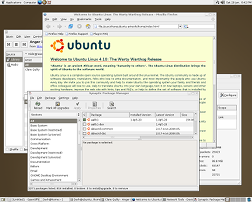
\includegraphics[scale=2.5]{cap01/Ubuntu410.png}
\caption{Curiosidade: Tela da Primeira Versão do Ubuntu a 4.10}
\end{figure}

Parte do problema estava na dificuldade do sistema, afinal de contas qual o motivo pelo qual teria que aprender a usar comandos de linha (também chamados de ``comandos de terminal'') tinha fugido do DOS e do Grande Porte exatamente por esse motivo, no Windows era tudo muito simples, clicar e instalar, clicar e remover, \textbf{Ctrl + C} e \textbf{Ctrl + V}.

Me parecia que o Linux não via assim e tudo deveria ser resolvido através do terminal. Era um tal de ``abre o terminal e digita o seguinte comando...'' e quando se precisava de um editor então? \textbf{Vi} saiu diretamente do inferno (inclusive está escrito na Bíblia: ``No terceiro dia do Regushad sete demônios trouxeram o Vi para a terra de Nod'' - Sei que é algum capítulo lá atrás), só pode ser, para alguém acostumado a um editor como \textbf{Bloco de Notas}, algo parecido com um editor da década de 60 só pode ter sido trazido pelo próprio ``coisa ruim'' (ou algum dos ``Cavaleiros do Apocalipse'' se prefere). O mundo Linux era algo para maluco ou Nerd de primeira categoria.

Quando resolvi mudar tive que enxergar esse novo ambiente através de novos olhos, Linux é um ambiente amigável, porém as pessoas é que continuam complicando com seus hábitos. O pensamento é o seguinte: ``Passo a vida inteira para aprender dezenas de comandos de terminal no Linux (outra eternidade para o Vi) e vou entregar todo esse conhecimento de mão beijada para um leigo? Não vou lucrar nada com isso?''

O que faz a força de uma linguagem? Quantas linguagens nascem e morrem todo santo dia? Já ouviu falar de \textbf{OAK}? Que tal \textbf{Algol}? Uma famosa criada pela Google denominada \textbf{Go}? Agora com certeza já ouviu falar de \textbf{Java}, \textbf{PHP}, \textbf{DotNet} e algumas outras (Até um tempo atrás se falasse de \textbf{R} ninguém saberia do que se trata - veja quando nasceu). O que dá a força de uma linguagem é o número de pessoas que a estão utilizando. Mesma coisa acontece a um sistema operacional, quanto mais pessoas o usarem mais ele vai se tornar conhecido e mais gente o usará. Partindo disso, o pensamento deveria ser assim: ``Se todas as pessoas conhecerem Linux, terei trabalho garantido fornecendo suporte, manutenção ou qualquer outra coisa que esteja no campo das habilidades aprendidas''. 

Era um usuário Windows (desde a versão 3.0), tive que adaptar alguns de meus hábitos para encarar esse novo mundo e reconhecer determinadas diferenças: \vspace{-1em}
\begin{itemize}[noitemsep]
 \item \textbf{Usuários Windows} não se veem em uma única pasta dentro do Sistema Operacional, se veem em todas as partes. A versão 98 até tentou criar este conceito com a pasta users (minhas músicas, bibliotecas, ...) porém ninguém usa isso. 
 \item \textbf{Usuários Linux} possuem claramente definido o conceito da pasta \textbf{home} (existe um comando para retornar ao diretório raiz: cd $\sim$), não que eles não possam atravessar essa fronteira, mas não existe o motivo para fazer isso.
 \item \textbf{Usuários Windows} não sabem quem são dentro do sistema, não existe esse conceito de ``usuário'', são simplesmente uma entidade no sistema e essa é a sua casa, são deuses, administradores, instalam e removem ao bel prazer.
 \item \textbf{Usuários Linux} sabem exatamente quem são (existe um comando para isso: whoami) e só usam o superusuário em ocasiões totalmente necessárias.
 \item \textbf{Usuários Windows} odeiam a janela de comandos, e muitos nem sabem os comandos MS-DOS, essa janela só é usada em último dos casos e por alguém que conhece muito do sistema.
 \item \textbf{Usuários Linux} acham que todos os problemas do sistema se resume a abrir a janela de terminal (sim, também existe um atalho para isso: Ctrl+Alt+T), é muito raro perguntar algo para uma pessoa deste mundo e não receber como resposta: abra a janela de terminal e...
 \item \textbf{Usuários Windows} instalam um software por impulso (ou para testá-lo ou para conhecê-lo) resultado que o sistema pode conter pastas que não são mais usadas ou lixo deixado por programas, a solução? Softwares de limpeza como o \textit{CCleaner} ou \textit{Glary Utilities}.
 \item \textbf{Usuários Linux} instalam somente programas necessários e reconhecidamente úteis. Pastas perdidas é quase uma heresia, sabem exatamente o que tem no sistema (e antes que pergunte sim, existe um comando para limpar a sujeira deixada por qualquer pacote: sudo apt autoclean).
\end{itemize}

Não estou dizendo que um grupo é melhor do que o outro, quero apenas mostrar as diferenças que tive que reconhecer para passar de um mundo ao outro. Porém muita coisa do Windows ainda estava grudada nas minhas células e disso não abriria mão: ``Quero sempre ter a facilidade de instalar um programa sem ter que usar uma janela de terminal''.

\subsection{Praticidade}\index{Conceitos Introdutórios}
Os defensores da janela de terminal possuem uma frase que adoro: ``É muito mais prático fazer as coisas pelo terminal''. Nunca poderia negar isso, como também acho muito mais prático trabalhar com modelos e macros para o LibreOffice/MS-Office, como acho muito mais prático usar a linguagem Bash/ScriptDos para resolver muitos problemas de processamento de muitas ações e como adoro as vezes programar em \textbf{Assembly}. O problema é o seguinte: quantas pessoas conhece que utiliza essas três ações práticas que citei?

Uma historinha que ainda não contei foi o drama que passei ao instalar o Ubuntu no meu \textbf{Notebook Dell} e isso porque a propaganda do site dizia \textit{Ubuntu Compatible}\footnote{Creio que desconheço a tradução correta dessa frase}. Tinha acabado de receber meu \textbf{Dell Inspirion 15R} e obviamente dei uma percorrida no Windows 8 pré-instalado só para sentir o que era, dois minutos depois estava formatando o computador e colocando o Ubuntu 14.04 (estou exagerando pois pensando bem acho que não chegou a dois minutos completos). Assim que terminei a instalação e reiniciei o computador, aconteceu que nem amarrado entrava no modo gráfico, pelo menos conseguia entrar em modo não gráfico e no meu desktop navegava na Internet para encontrar a solução.

Após tentar de tudo o que os sites tinham descritos sobre esse problema (que era mais comum do que pensava). Consegui a solução\footnote{Como forma de ajudar outras pessoas publiquei essa dica no mesmo dia que consegui a solução} que no meu caso envolvia instalar os drivers do \textbf{Ubuntu 13.10}. Foi a seguinte sequencia de comandos que tive de digitar:

1. Verificar a compatibilidade com o VGA: \\
{\ttfamily\$ lspci | grep VGA}

2. Baixar o drive compatível do Ubuntu 13.10. \\
{\ttfamily\$ cd $\sim$/ \\
\$ wget https://download.01.org/gfx/ubuntu/13.10/main/pool/main/i/ \\ intel-linux-graphics-installer/ \\ intel-linux-graphics-installer\_1.0.4-0intel1\_amd64.deb
\$ sudo apt install ttf-ancient-fonts
\$ sudo dpkg -i intel-linux-graphics-installer\_1.0.4-0intel1\_amd64.deb}

E pronto, após dois dias tudo tinha se resolvido. Agora vamos raciocinar um pouco, apenas descobri a solução porque queria instalar o Ubuntu e já estava convencido que não usaria mais o Windows. Porém sobra uma pergunta: E se tivesse apenas testando o Linux para me decidir qual sistema colocar? Acredita realmente que ficaria tentando todas as formas possíveis até ter essa solução ou simplesmente abandonaria tudo e usaria o Windows (e seria bem mais fácil). 

Não estou dizendo que a janela de terminal não é prática, mas acho que não devemos confundir o termo \textbf{praticidade} com \textbf{facilidade}. O \textbf{Clipper} era uma linguagem muito prática de se usar, fácil de aprender mas morreu porque o mundo mudou e as pessoas começaram a usar o modo gráfico. Aí surgiu o \textbf{Delphi} um ambiente muito prático para se criar as novas janelas gráficas, mas morreu porque o mundo mudou e a programação passou a ser voltada para a Web. Coisas práticas morrem, simples assim. Não quero ver o Linux morrer, ao contrário quero vê-lo crescer cada vez mais e ganhar novos adeptos, só que para isso devemos deixar de lado certos hábitos (assim como abandonei o Clipper e o Delphi) e nos dedicarmos ao que realmente importa para o usuário leigo.

Falei muito do meu Note, mas no meu desktop também já tive problemas em instalar a placa gráfica da Intel, até encontrar a correta na qual foi instalada com os seguintes comandos: \\
{\ttfamily\$ sudo apt install intel-linux-graphics-installer \\
\$ sudo apt install xserver-xorg-video-intel \\
\$ sudo add-apt-repository ppa:xorg-edgers/ppa \\
\$ sudo apt upgrade \\
\$ sudo modprobe -r psmouse \\
\$ sudo modprobe psmouse proto=imps}

Recomendo, antes de se aventurar na instalação do Linux, saiba exatamente todo conteúdo do seu hardware para evitar qualquer problema (coisa que normalmente não interessa ao usuário Windows).

\section{Por que escolhi o Ubuntu?}\index{Conceitos Introdutórios}
Primeiro gostaria de responder uma pergunta sobre o que é Linux? Muita gente acha que é um Sistema Operacional (aposto que também pensou isso alguma vez) pois saiba que não é, Linux é um \textbf{Kernel}. O sistema operacional consiste em uma escolha das milhares de distribuições existentes que foram criadas em cima deste Kernel.

Para entrar no mundo Linux primeiro é necessário escolher uma família, e quais são as disponíveis? E o que significa cada uma delas? Com a ajuda do material da \textbf{Linux Foundation} permita-me explicar e ajudá-lo a entender como é esse mundo.
\begin{figure}[H]
	\centering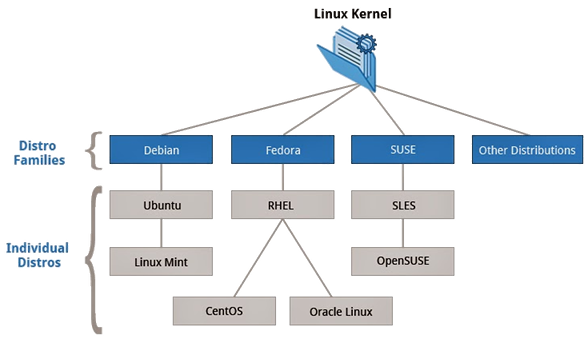
\includegraphics[scale=2.5]{cap01/familias.png}
	\caption{Famílias mais conhecidas do Linux}
\end{figure}

De pronto observamos que todas as distros do Linux vem de um Kernel (entenda isso como o núcleo do Sistema Operacional ou simplesmente O Linux) único e que pode ser atualizado sem que para isso seja necessário mudar a versão da sua distribuição, e isso é muito bom pois o que muda é apenas a forma como o usuário final enxerga sua máquina e pode configurá-la ao seu jeito e escolher a distribuição que mais lhe agradar.

Existem milhares de distribuições (ou simplesmente distros)? O pior, cada uma é tão excelente quanto sua concorrente e isso confunde um leigo nesse mundo. Vamos resumir e ficar apenas com algumas delas e realizar a escolha devido a necessidade.
\begin{description}
 \item[Família Debian] Debian serve de base para várias outras distribuições, incluindo Ubuntu, que por sua vez serve de base para Linux Mint e outros (Edubuntu por exemplo). É comumente utilizada tanto em servidores como em desktops. Debian é um projeto de código aberto puro e se concentra em um aspecto fundamental: \textbf{estabilidade}. Também fornece o maior e mais completo repositório de softwares para seus usuários. Usa o gerenciador de pacotes \textbf{apt}\footnote{É um projeto amplo, cujos planos originais incluía uma interface gráfica. Tem por base uma biblioteca que contém as aplicações principais e um instalador em linha de comando} com base no DPKG para instalar, atualizar e remover pacotes no sistema.
 \item[Família Fedora] Fedora forma a base para RHEL\footnote{Red Hat Enterprise Linux}, CentOS, Scientific Linux e Oracle Linux. Essa família contém significativamente mais software do que a versão empresarial da Red Hat. Uma razão para isso é uma comunidade diversificada e envolvida na construção do Fedora; e não apenas uma empresa. Normalmente o CentOS é usado para atividades como demonstrações e laboratórios, pois está disponível sem nenhum custo para o usuário final e possui um ciclo de lançamento mais longo do que o Fedora (que lança uma nova versão a cada seis meses ou mais), sendo bem mais estável. Já o RHEL é a distribuição mais popular em ambientes corporativos. Usa o gerenciador de pacotes \textbf{yum} com base no RPM para instalar, atualizar e remover pacotes no sistema
 \item[Família SUSE] A relação entre o SUSE, SLES\footnote{SUSE Linux Enterprise Server} e OpenSUSE é semelhante à descrita anteriormente. OpenSUSE é a distribuição de referência desta família para os usuários finais, sem nenhum custo. Os dois produtos são extremamente semelhantes, e qualquer material deste pode normalmente ser aplicada ao SLES sem nenhum problema. Usa o gerenciador de pacotes \textbf{zypper} com base no  RPM para instalar, atualizar e remover pacotes no sistema. Também inclui o aplicativo \textbf{YaST} (outra ferramenta do Sistema) para fins de administração.
\end{description}

\begin{dica}[Empacotamento APT] \textit{Advanced Packaging Tool} é um conjunto de ferramentas usadas pelo GNU/Linux Debian e suas respectivas derivações, entre eles o Ubuntu, para administrar os pacotes .deb de uma forma automática, deste modo quando um programa é instalado o APT instala e/ou atualiza também todos os pacotes que são necessários para o correto funcionamento do programa.
	
O Ubuntu 18.04 eliminou a necessidade, em muitos casos, do comando: \\
{\ttfamily\$ sudo apt update}
\end{dica}

Resumidamente, temos as seguintes distribuições para escolher: \vspace{-1em}
\begin{itemize}[noitemsep]
 \item Ubuntu, distro voltada ao ``povão'', ou seja, para a grande maioria dos usuários, fácil e acessível, procura se tornar a mais amigável e estável possível.
 \item Linux Mint, é a distribuição concorrente direta do Ubuntu, colocando em termos práticos digamos que procura ser a versão mais bonita e elegante. 
 \item RHEL ou Oracle Linux, duas grandes empresas por trás dessas distribuições e voltada para um público/máquinas totalmente profissional, ou seja, exclusivamente para empresas. Pretende rodar um Servidor de Dados, montar um repositório para nuvem, gerenciar sua empresa através de um ERP, opte por uma dessas.
 \item CentOS ou Fedora, ambas garantem um bom lugar no mercado graças a distribuição RHEL, o que tem a ver? No servidor da empresa existe a RHEL só que no consultor que fornece a manutenção vai ter provavelmente uma dessas duas distribuições.
 \item Slackware ou Debian, boa parte das distribuições citadas anteriormente tiveram sua origem em uma dessas duas, são as mais ``geeks'' e voltadas apenas para o usuário mais profissional.
\end{itemize}

\subsection{Minha Distribuição}\index{Conceitos Introdutórios}
Para minha máquina optei pela distribuição \textbf{Ubuntu}e iniciei minha jornada na versão 14.04. Esta distribuição tem por objetivo proporcionar uma boa experiência entre a estabilidade a longo prazo e facilidade de uso. Recebe a maior parte de seus pacotes da parte estável da Debian, mas também tem acesso a um repositório de software muito grande. \\[3mm]
Atualmente retornou a interface Gnome, porém difere visualmente da interface do padrão Debian, bem como de outras distribuições (boa parte graças a heranças do ambiente gráfico Unity - Utilizado até a 16.10). Além disso tudo, sua instalação e manutenção foram as mais simples e intuitivas que já realizei.
\\[3mm]
\begin{dica}[Começando agora?] Recomendo que veja essa coletânea de vídeo do DioLinux se ainda sente dificuldade em entender alguma coisa:
 \begin{itemize}[noitemsep]
   \item \url{https://www.youtube.com/watch?v=5nX4UFQt_JQ} O que é Linux? Conheça as principais distribuições
   \item \url{https://www.youtube.com/watch?v=ikfLh2izqAA} Qual a melhor distribuição Linux para Iniciantes?
   \item \url{https://www.youtube.com/watch?v=z4QeIULKpKo} Como baixar o Ubuntu?
   \item \url{https://www.youtube.com/watch?v=ShH2U4D5tjM} Como instalar o Ubuntu 14.04 corretamente (Canal RBTech)
 \end{itemize}
\end{dica}

Ubuntu é uma palavra masculina ou feminina? Fala-se ``O Ubuntu'' quando nos referimos ao Sistema Operacional Ubuntu, como também podemos usar ``A Ubuntu'' ao falarmos da Distribuição, então não se assuste se durante esse livro usar os dois termos.

% Final do Capítulo
\clearpage